\documentclass[11pt,twoside]{article}

\usepackage{paperlighter}

% Recommended, but optional, packages for figures and better typesetting:
\usepackage{microtype}
\usepackage{graphicx}
\usepackage{subfigure}
\usepackage{booktabs} % for professional tables

% Attempt to make hyperref and algorithmic work together better:
\newcommand{\theHalgorithm}{\arabic{algorithm}}


% For theorems and such
\usepackage{amsmath}
\usepackage{amssymb}
\usepackage{mathtools}
\usepackage{amsthm}

% if you use cleveref..
\usepackage[capitalize,noabbrev]{cleveref}

%%%%%%%%%%%%%%%%%%%%%%%%%%%%%%%%
% THEOREMS
%%%%%%%%%%%%%%%%%%%%%%%%%%%%%%%%
\theoremstyle{plain}
\newtheorem{theorem}{Theorem}[section]
\newtheorem{proposition}[theorem]{Proposition}
\newtheorem{lemma}[theorem]{Lemma}
\newtheorem{corollary}[theorem]{Corollary}
\theoremstyle{definition}
\newtheorem{definition}[theorem]{Definition}
\newtheorem{assumption}[theorem]{Assumption}
\theoremstyle{remark}
\newtheorem{remark}[theorem]{Remark}

% Todonotes is useful during development; simply uncomment the next line
%    and comment out the line below the next line to turn off comments
%\usepackage[disable,textsize=tiny]{todonotes}
\usepackage[textsize=tiny]{todonotes}


\begin{document}

\lightertitle{Case Study: How Does a Bike-Share Navigate Speedy Success?}

\lighterauthor{Phuc Nguyen}

\lighteraddress{$^\dagger$}{540 North Avenue, unit D, Fort Lee NJ 07024}

\lighteremail{n.hong.phuc@gmail.com}

In this report, we analyze the data of the bike-sharing company Cyclistic in Chicago. This latter company is looking for ways to convert casual users of its service into annual members, because the latter are much more profitable to the company than the casual riders. We will follow the six steps of the data analysis process: ask, prepare, process, analyze, share and act.

\section{Ask}
As mentioned in the introduction, the business task is to figure out how convert casual riders into members. To answer this question, we will dive into the data from the past 12 months, to identify ways in which members and casual riders use the bike-sharing service differently. This analysis will help us make recommendations for how to organize a marketing campaign to convert the casual riders. For example, if we see that casual riders tend to use the service more often at a particular time of the day, or in a particular area of Chicago, then we want to focus our marketing efforts on such times and places.

\section{Prepare}
The data sources we used are the historical trip data of Cyclistic. The data has been made publicly available by Motivate International Inc. under the license which can be found here https://ride.divvybikes.com/data-license-agreement. No personally identifiable information is in the data however, due to data-privacy issues.

\section{Process}
To make sure that the data is clean, we have performed several consistency checks (using SQL). First, we checked that all the ride IDs listed in the ride\_ID column are mutually distinct, and that they all have the same length. Secondly, we checked that the column rideable\_type only takes 3 value: electric bike, classic bike and docked bike, which also makes sense. Thirdly, we make sure that the datetimes listed in the columns started\_at and ended\_at are sensible (by checking that they all correspond to one of the seven days of the week, and also by checking that they all belong to the month they are supposed to belong to). Fourthly, we made sure that the latitudes and longitudes of the stations are sensible by plotting them on a map of Chicago using Tableau. Fifthly, we made sure that the column member\_casual only takes two values: member and casual.\\
Overall, the data seem clean, and we have not identified any dirty data.

\section{Analyze}
We found that casual riders tend to ride for a longer period of time (typically two and a half times to three times longer). This suggests that casual riders use their bikes for sightseeing or tourism purposes, whereas members use their bikes to commute to work.\\ Furthermore, if we break down the average trip duration by season of the year, we see that for both members and casual riders, the average trip duration is the shortest in the winter, and longer in the three other seasons. This is not surprising because people are not inclined to bike during the cold winter months. However, the difference between the winter and the 3 other seasons is more pronounced for casual riders than for members, suggesting that indeed casual riders use the bikes for leisures whereas members bike to commute to work. Indeed, activities such as tourism pick up strongly in the warmer months of the year, whereas commuting to work should be expected to be more or less constant year-round.\\
Next, we focus on the type of bike most commonly used by casual riders and members. We find that, until recently, the classic bike is the favorite type among both casual riders and members. However, more recently the electric bike has become the favorite type among casual riders. Among the members, the classic bike remains the favorite bike type, although electric bike is gaining in popularity among members as well.\\
Next, we focus on the breakdown of the number of rides by day of the week. We see that the casual riders tend to ride more frequently at weekends (Saturday and Sunday), whereas the members tend to ride more frequently during the business days. This again supports the hypothesis that the casual riders ride for tourism or leisure, whereas the members ride for work commute. Furthermore, by breaking down the number of trips into hours of the day, we see further evidence that member rides are work-related, because there is a peak in the number of rides among members around rush hour in the morning (and there is no such peak for the number of rides among casual riders).\\
Finally, it is also interesting to investigate the geographic distribution of trips made by casual riders and members. We find that trips made by casual riders are more evenly spread out across Chicago than trips by members. For example, within the central area of Chicago, trips by members are most concentrated in the Loop area.

\section{Share}
In Figure 1, we show a bar chart which shows that the casual riders indeed take more time with their rides than the members. We have chosen to show data for four different months (which are representative of the four seasons of the year) separately, to convey a sense of seasonal variation of the data.
\begin{center}
\begin{figure}
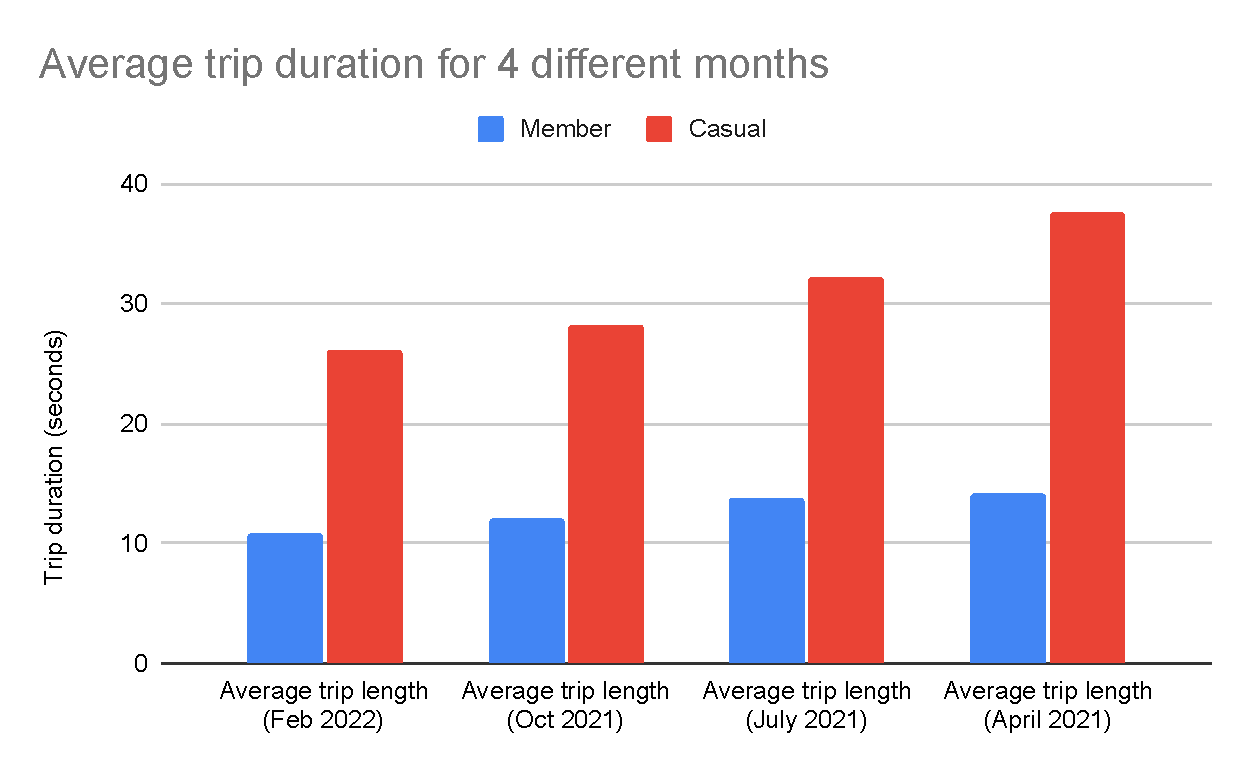
\includegraphics[width=12cm, height=8cm]{Average trip duration.pdf}
\caption{Average trip duration.}
\end{figure}
\end{center}
In figure 2, we show another collection of bart charts, which shows that electric bike is becoming more and more popular among both casual riders and members, and has even become the favorite type of bike among casual riders.
\begin{center}
\begin{figure}
\begin{subfigure}{}
  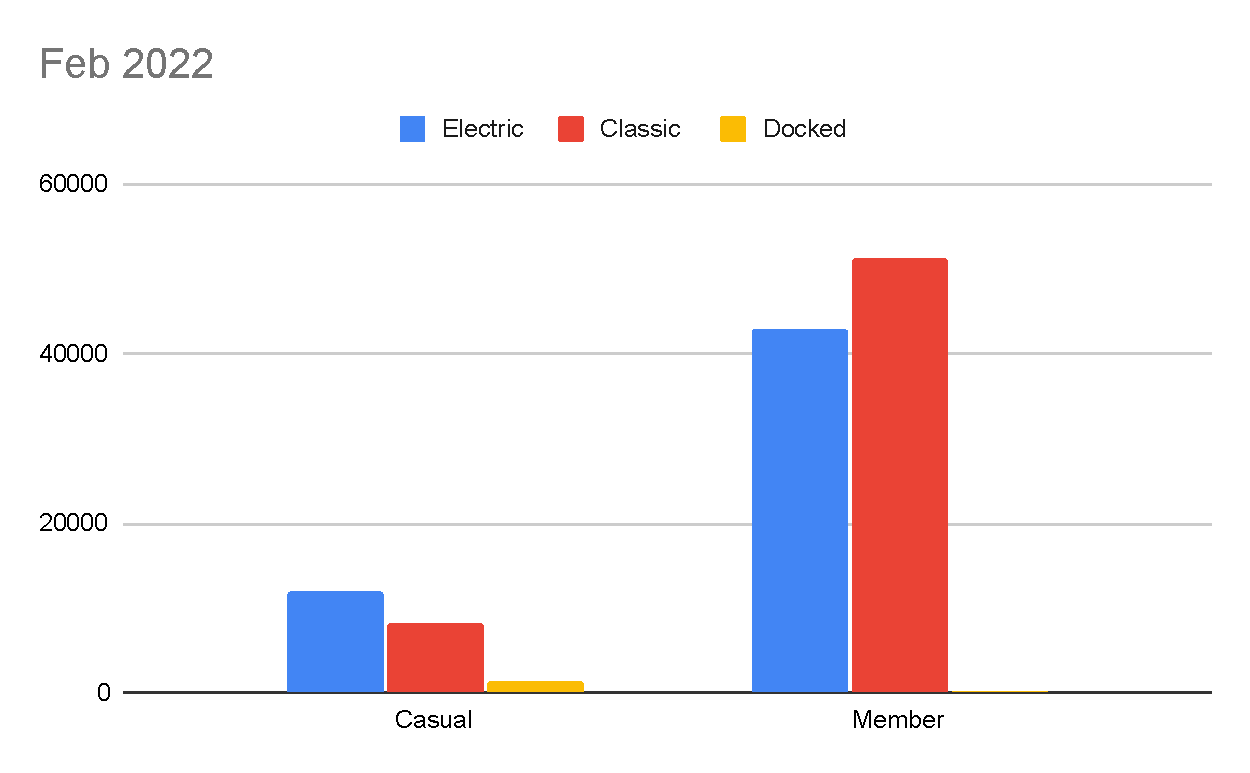
\includegraphics[width=.5\linewidth]{Feb2022RideBreakdown}
\end{subfigure}%
\begin{subfigure}{}
  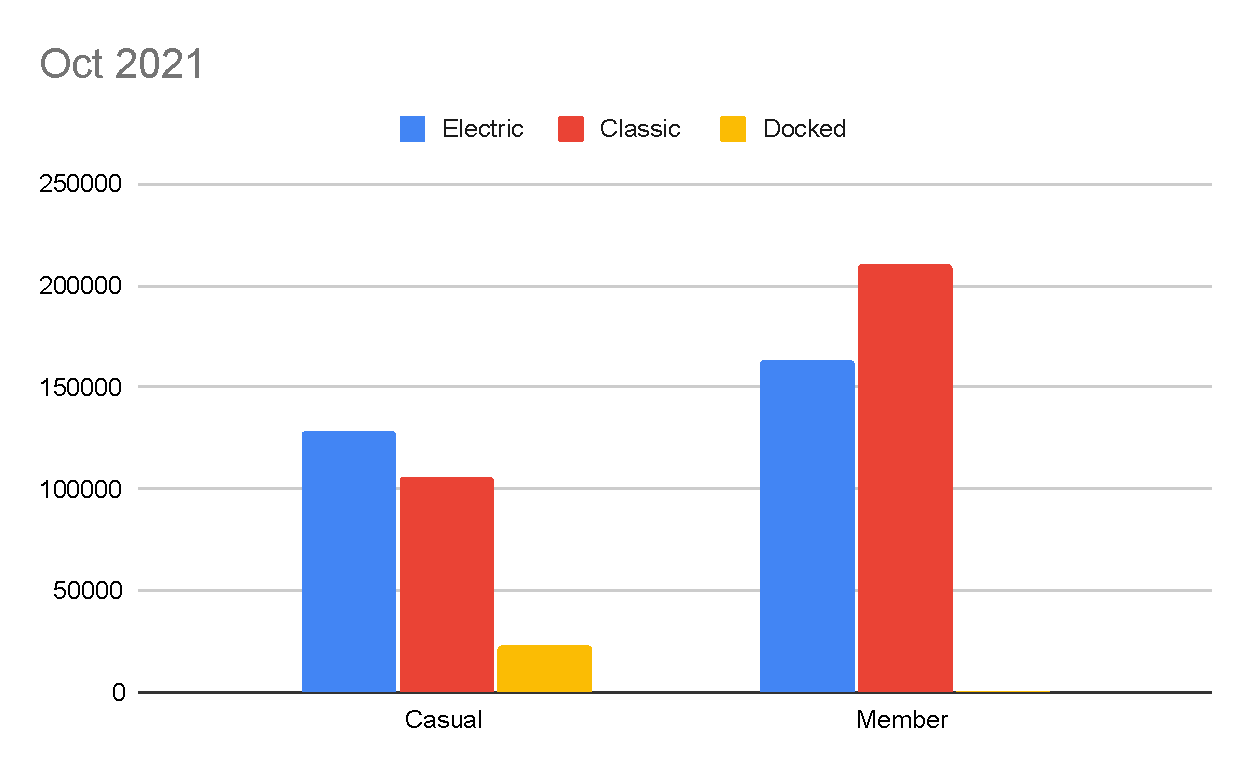
\includegraphics[width=.5\linewidth]{Oct2021RideBreakdown}
\end{subfigure}\\
\begin{subfigure}{}
  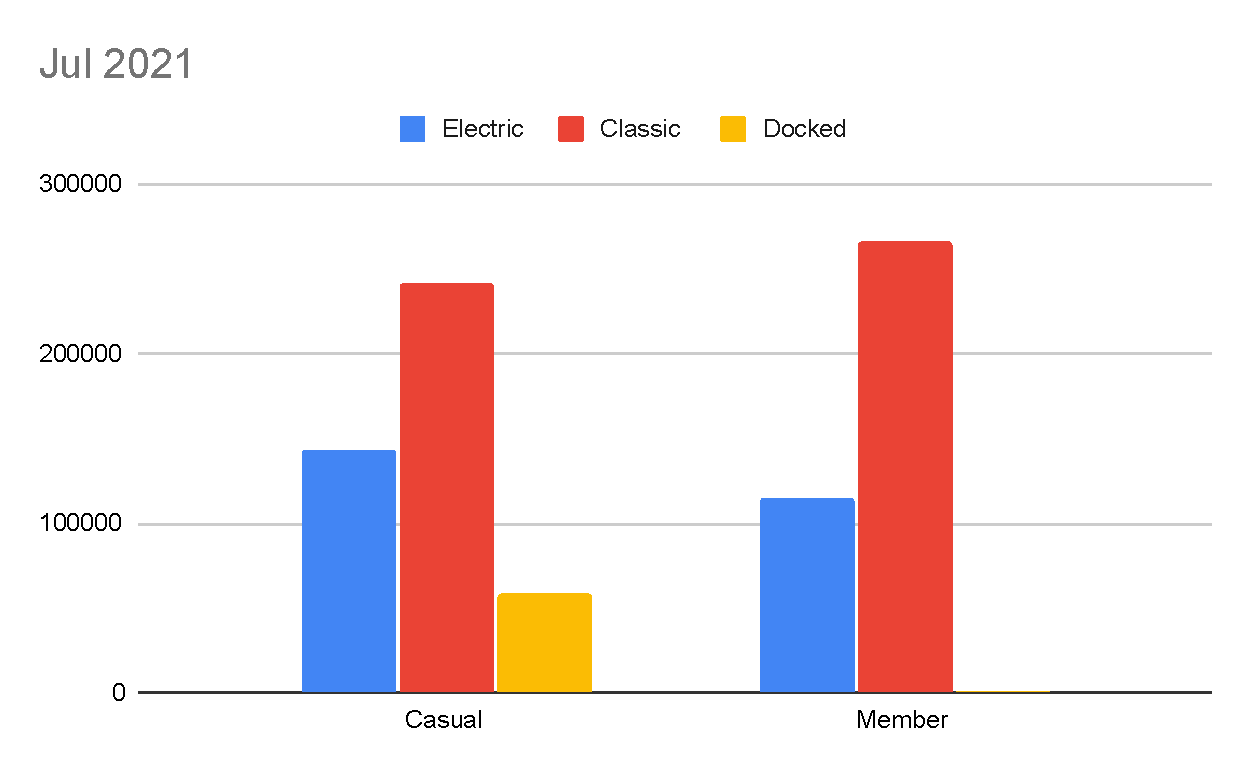
\includegraphics[width=.5\linewidth]{Jul2021RideBreakdown}
\end{subfigure}
\begin{subfigure}{}
  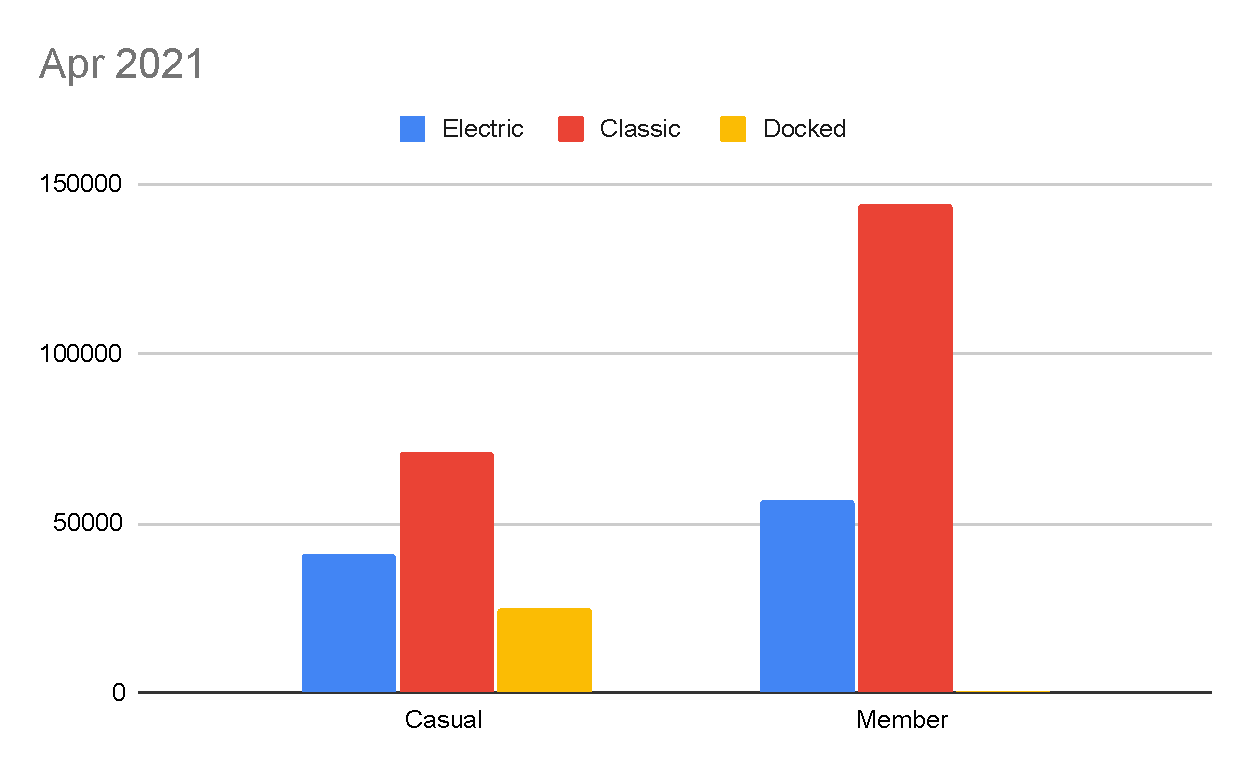
\includegraphics[width=.5\linewidth]{Apr2021RideBreakdown}
\end{subfigure}
\caption{Number of rides, broken down by type of bike and type of membership. Each of the four panels represents a season in the year.}
\label{fig:RideBreakdown}
\end{figure}
\end{center}
In Fig. 3 below, we break down the number of rides into the membership type and the day of the week.
\begin{center}
\begin{figure}
\begin{subfigure}{}
  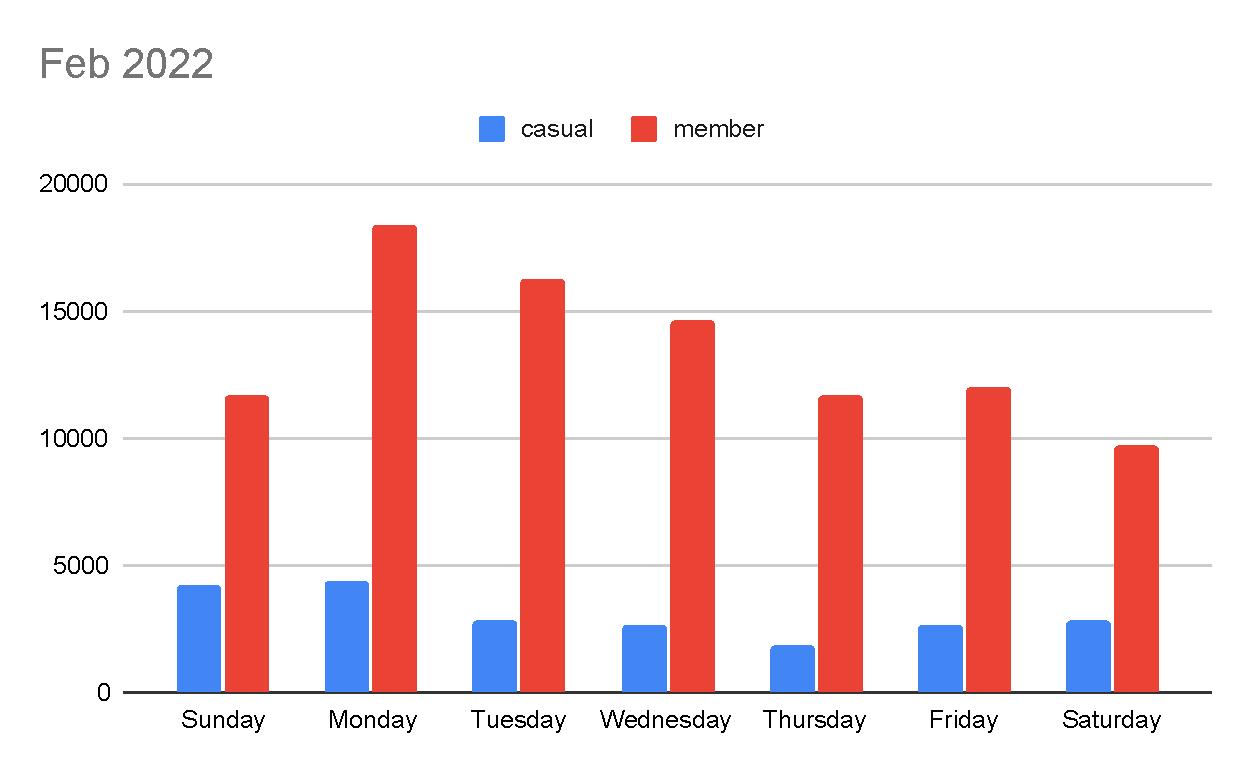
\includegraphics[width=.5\linewidth]{Feb 2022}
\end{subfigure}%
\begin{subfigure}{}
  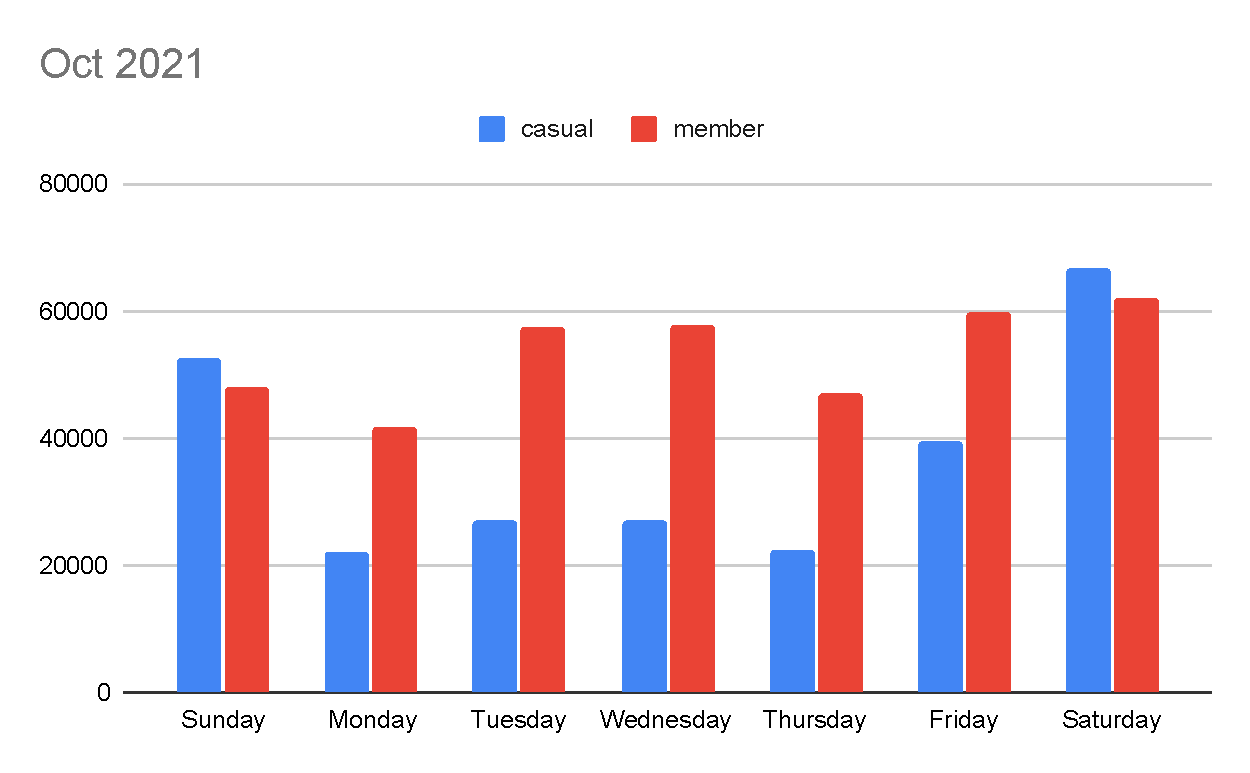
\includegraphics[width=.5\linewidth]{Oct 2021}
\end{subfigure}\\
\begin{subfigure}{}
  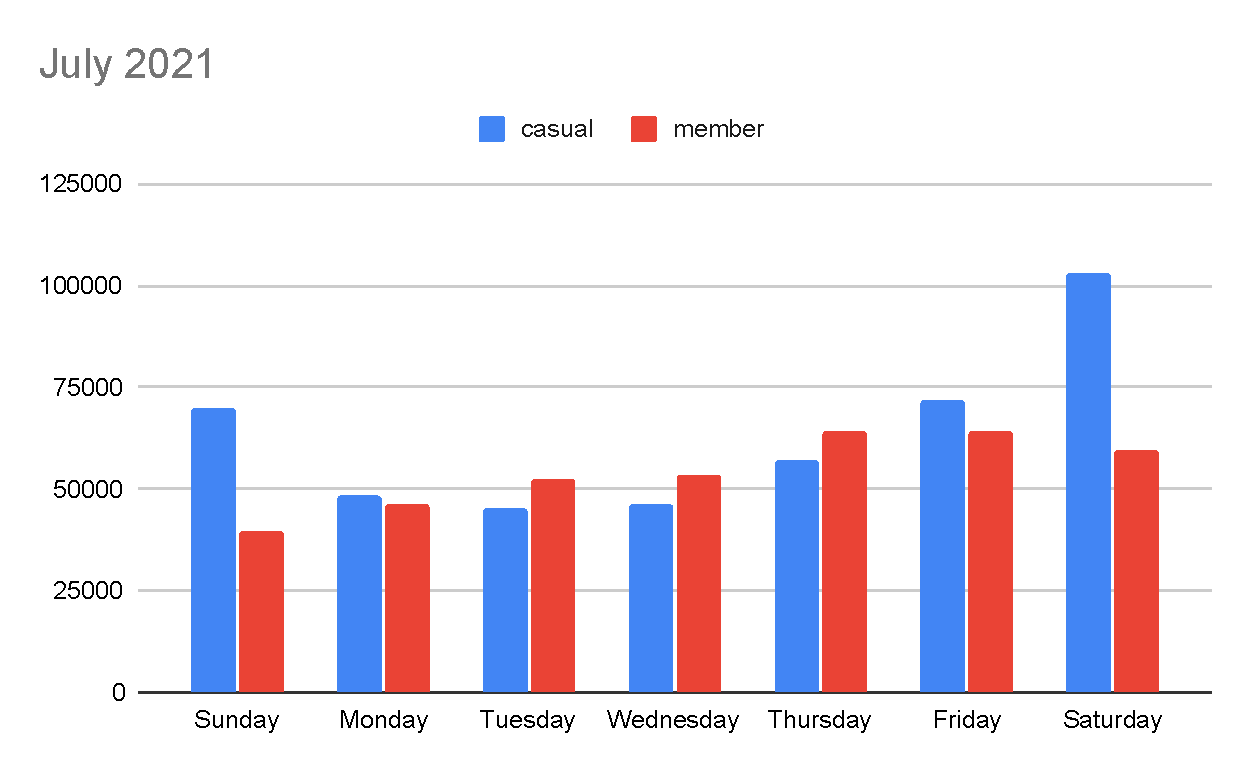
\includegraphics[width=.5\linewidth]{July 2021}
\end{subfigure}
\begin{subfigure}{}
  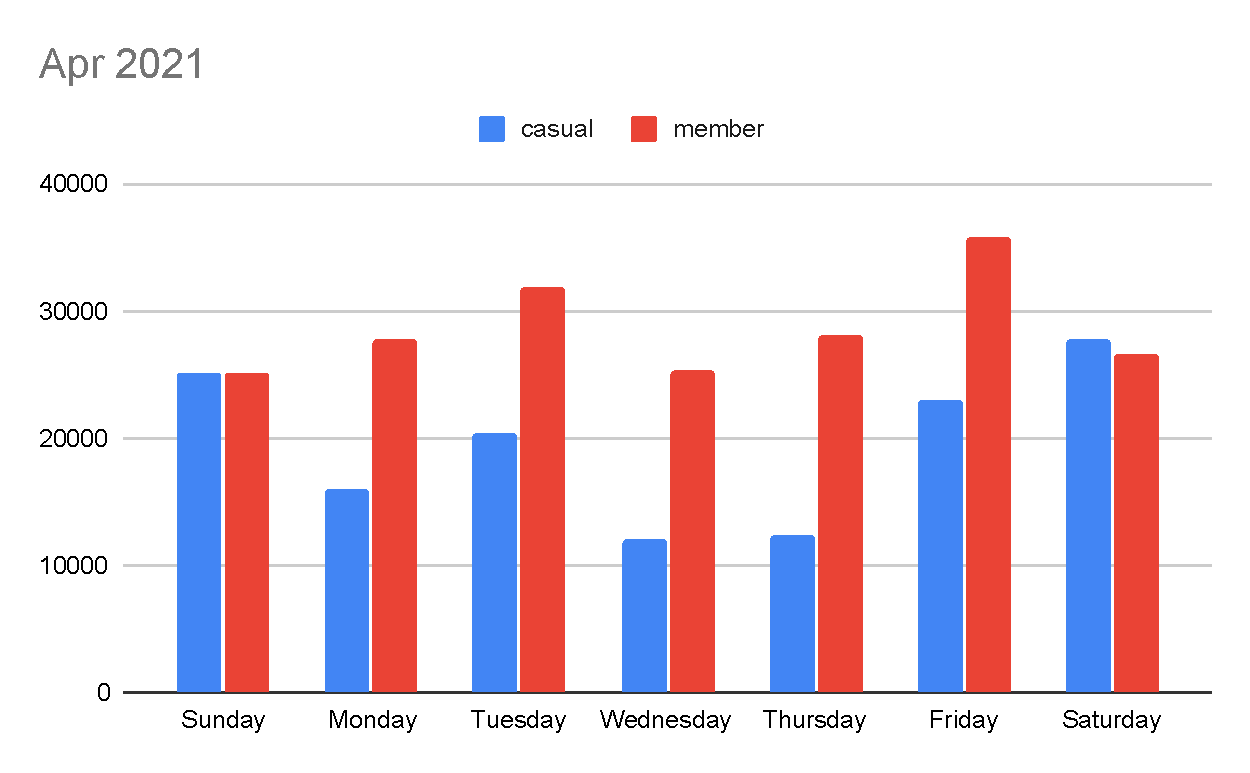
\includegraphics[width=.5\linewidth]{Apr 2021}
\end{subfigure}
\caption{Number of rides, broken down by day of the week and type of membership. Each of the four panels represents a season in the year.}
\label{fig:RideBreakdown}
\end{figure}
\end{center}
In Fig. 4 below, we focus on the data in April 2021, and break it down by hour of the day and by membership type.
\begin{center}
\begin{figure}
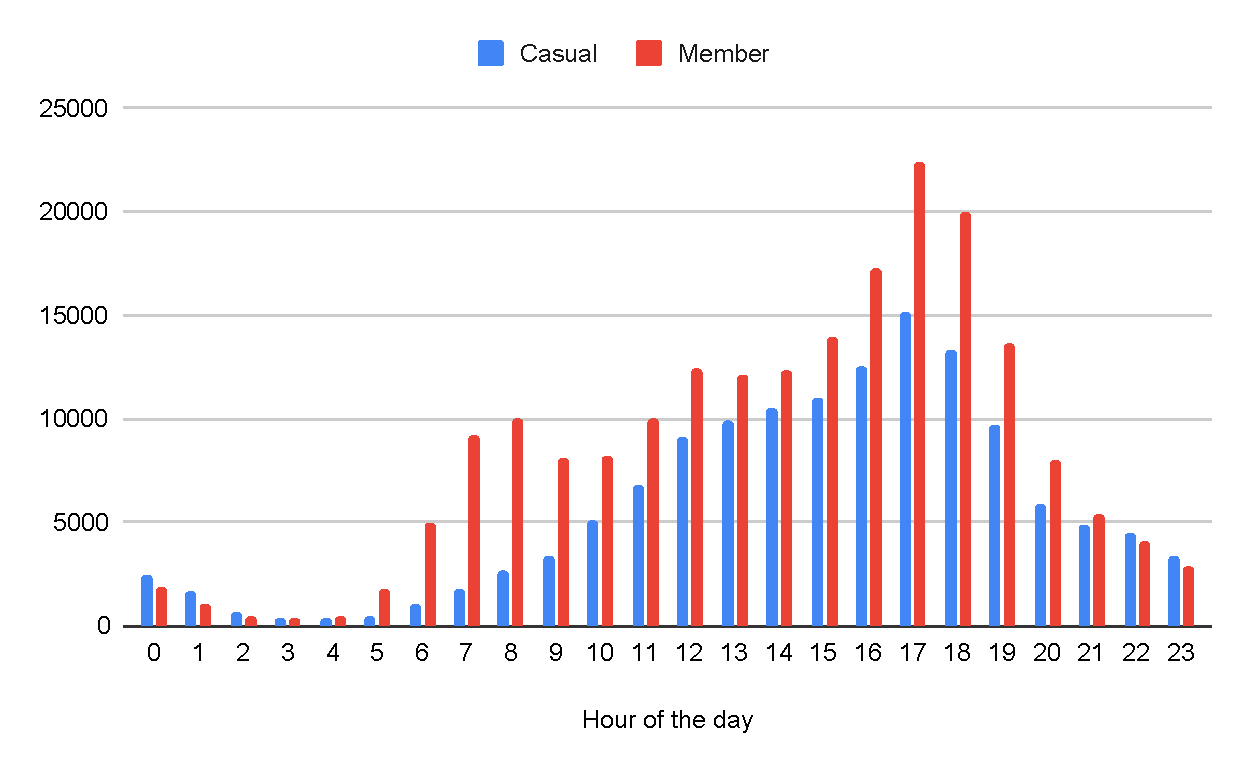
\includegraphics[width=12cm, height=8cm]{BreakdownByHour.pdf}
\caption{Breakdown of number of trips in April 2021 by hour of the day and membership type.}
\end{figure}
\end{center}
Finally, in figure 5 below, we present the geographic distribution of starting points of trips in Feb 2021.

\begin{center}
\begin{figure}
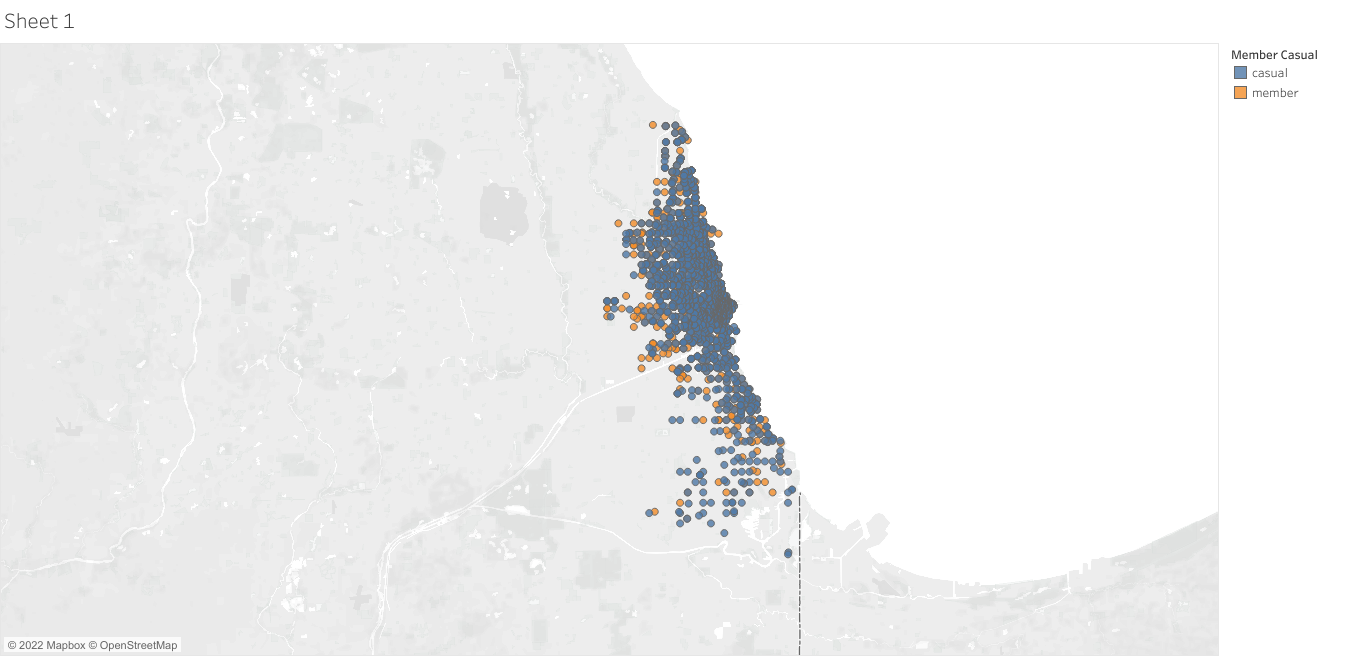
\includegraphics[width=15cm, height=8cm]{Sheet 1}
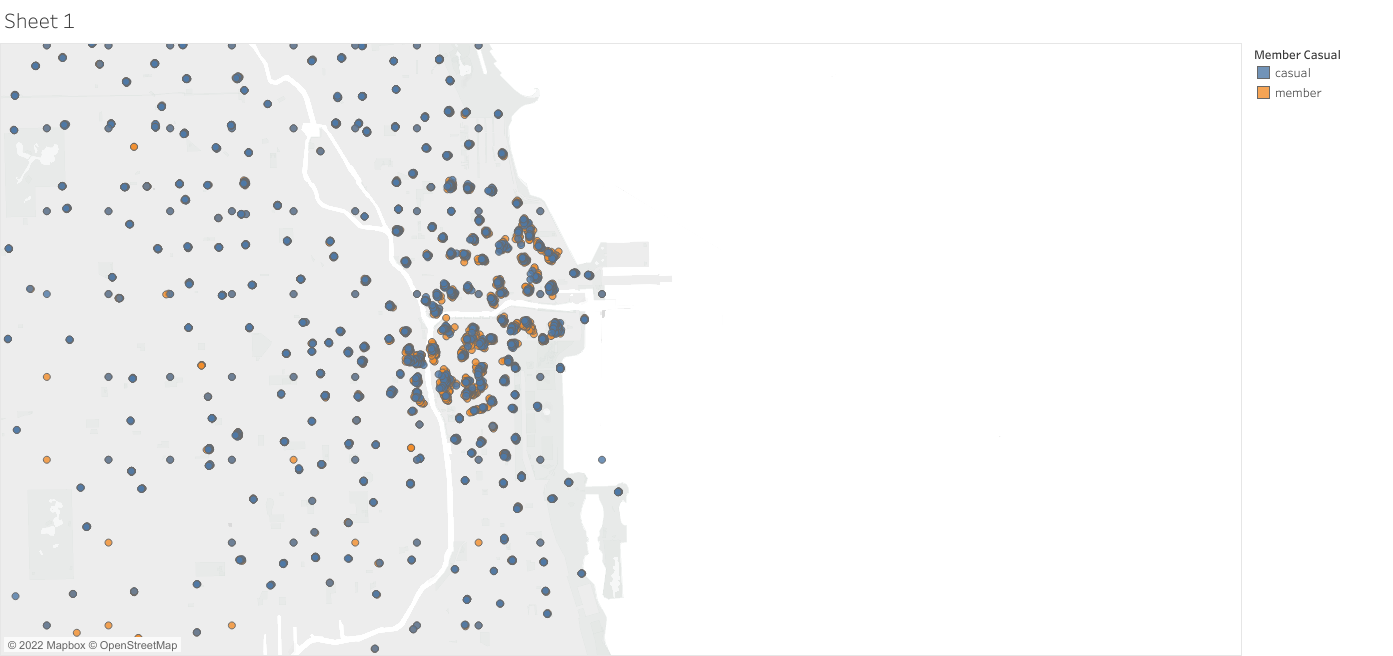
\includegraphics[width=15cm, height=8cm]{Sheet 2}
\caption{Geographic distribution of starting stations of trips in Feb 2021. Blue points correspond to trips by casual riders, and oragne points correspond to trips by members.}
\end{figure}
\end{center}

\section{Act}
Based on the findings above, we make the following 3 recommendations:
\begin{itemize}
    \item The marketing campaign to try to win more members should be targeted at riders who rent electric bikes, or who ride for longer time periods, because such riders tend to be casual riders. Cyclistic could for example offer discounts for signing up for membership to such riders.
    \item In the winter, the number of rides is lower than in the warmer months of the year, obviously because of the colder weather. The marketing campaign can offer discounts for signing up for membership during the winter months, to encourage more people to ride bikes.
    \item Based on the geographic distribution of rides, the marketing campaign can focus on those areas of Chicago where there are currently fewer rides by members, for example the area near downtown Chicago outside the Loop.
\end{itemize}

\end{document}